\documentclass[10pt, aspectratio=169]{beamer}
\usetheme{Warsaw}
\usecolortheme{beaver}

\definecolor{darkred}{rgb}{0.54,0,0}

\usepackage{caption}
\captionsetup{labelfont={color=darkred,bf}}
\captionsetup[figure]{name=Рис.}
\captionsetup[table]{name=Табл.}

\setbeamercolor{structure}{fg=darkred} % itemize, enumerate, etc
\setbeamertemplate{caption}[numbered]
\setbeamertemplate{navigation symbols}{}

\setbeamertemplate{footline}{
	\leavevmode%
	\hbox{%
		\begin{beamercolorbox}[wd=.35\paperwidth,ht=2.25ex,dp=1ex,center]{author in head/foot}%
			\usebeamerfont{author in head/foot}\insertshortauthor
		\end{beamercolorbox}%
		\begin{beamercolorbox}[wd=.575\paperwidth,ht=2.25ex,dp=1ex,center]{title in head/foot}%
			\usebeamerfont{title in head/foot}\insertshorttitle
		\end{beamercolorbox}%
		\begin{beamercolorbox}[wd=.075\paperwidth,ht=2.25ex,dp=1ex,right]{date in head/foot}%
			\insertframenumber{} / \inserttotalframenumber\hspace*{2ex}
	\end{beamercolorbox}}%
	\vbox{}%
}

\usepackage{amsmath,amsthm,amssymb}
\usepackage[T1,T2A]{fontenc}
\usepackage[utf8]{inputenc}
\usepackage[english,russian]{babel}
\usepackage{array}

\usepackage{tikz}
\usepackage{dsfont}
\usepackage{cancel}
\usepackage{ulem}

\usepackage{graphicx}%Вставка картинок правильная
\usepackage[caption=false]{subfig}
\usepackage[export]{adjustbox}
\usepackage{float}%"Плавающие" картинки
\usepackage{wrapfig}%Обтекание фигур (таблиц, картинок и прочего)

\usepackage{listings}

\usepackage{hyperref}
\hypersetup{
	colorlinks = true,
	linkcolor = black,
	filecolor = black,      
	urlcolor = black,
	citecolor = black,
	pdftitle={Выпускная квалификационная работа, Андреев Иван Николаевич, 22.Б27-фз.},
	% pdfpagemode=FullScreen,
}
\usepackage{multirow}

\newcommand{\Rarr}{\Rightarrow}
\newcommand{\rarr}{\rightarrow}
\newcommand{\Lrarr}{\Leftrightarrow}
\newcommand{\lrarr}{\leftrightarrow}
\newcommand{\ths}{\thinspace}
\newcommand{\ptl}{\partial}
\newcommand{\defis}{— }
\newcommand{\degg}{º}
\newcommand*\circled[1]{\tikz[baseline=(char.base)]{
		\node[shape=circle,draw,inner sep=2pt] (char) {#1};}}

\definecolor{codegreen}{rgb}{0,0.6,0}
\definecolor{codegray}{rgb}{0.5,0.5,0.5}
\definecolor{codepurple}{rgb}{0.58,0,0.82}
\definecolor{backcolour}{rgb}{0.95,0.95,0.92}

\lstdefinestyle{mystyle}{
	backgroundcolor=\color{backcolour},   
	commentstyle=\color{codegreen},
	keywordstyle=\color{magenta},
	numberstyle=\tiny\color{codegray},
	stringstyle=\color{codepurple},
	basicstyle=\ttfamily\footnotesize,
	breakatwhitespace=false,         
	breaklines=true,                 
	captionpos=b,                    
	keepspaces=true,                 
	numbers=left,                    
	numbersep=5pt,                  
	showspaces=false,                
	showstringspaces=false,
	showtabs=false,                  
	tabsize=2
}

\lstset{style=mystyle}

\usepackage{mhchem}
\usepackage{chemfig}

\usepackage{ragged2e}

%Information to be included in the title page:
\title[Электронно-возбужденные состояния в кластерах меди, защищенных тиолятами]
{Электронно-возбужденные состояния в кластерах меди, защищенных тиолятами}

\subtitle{Выпускная квалификационная работа.\\ Направление: 03.03.01 «Прикладные физика и математика» (CB.5009.2022)}

\author[Андреев Иван Николаевич (22.Б27-фз)]{Выполнил: \textbf{Андреев Иван Николаевич} (группа 22.Б27-фз) \\ Научный руководитель: к.х.н., с.н.с. \textbf{Буглак Андрей Андреевич}}

\institute{Санкт-Петербургский государственный университет, Физический факультет \\ Кафедра молекулярной биофизики и физики полимеров}

\titlegraphic{
\includegraphics[width=9cm]{Logo_new.jpg}}

\date{г. Санкт-Петербург, 2026}

\begin{document}

\begin{frame}[plain]
	\titlepage
\end{frame}	

\begin{frame}{Введение. Металлические нанокластеры.}
	\begin{columns}
		\column{0.4\textwidth}
		
		\begin{alertblock}{Металлические нанокластеры}
			\justify
			 \small — объекты, состоящие из единиц–сотен атомов металлов. Благодаря малым размерам, они демонстрируют дискретные молекулярно-подобные энергетические уровни. Это делает возможным их детектирование при помощи фотометрических методов измерения поглощения, комбинационного рассеяния и люмиинесценции.
		\end{alertblock}
		\vfill
		\justify
		Нанокластеры как таковые требуют стабилизации лигандами, в качестве которых выбираются органические соединения: аминокислоты, ДНК, олигонуклеотиды, тиолы и пр. 
		
		\column{0.6\textwidth}
		
		\begin{figure}
			
\includegraphics[width=0.7\linewidth]{pictures/Cu3L2.png}
			\caption{\centering \scriptsize Трёхатомный кластер меди с метилтиогруппой.}
		\end{figure}
		
	\end{columns}
\end{frame}

\begin{frame}{Введение. Тиолы.}
	\justify
	\textbf{Тиолы и тиоляты} — органические соединения с функциональной тиольной/тиолятной группой (т.е. молекулы вида RSH/RS-, где R — органический радикал). К тиолам относятся множество важных веществ в организме человека:
	\begin{itemize}
		\item \textbf{Глутатион (GSH)} — главный внутриклеточный антиоксидант, наиболее важное тиоловое соединение клеток;
		\item \textbf{Цистеин} — серосодержащая аминокислота, необходимая для синтеза белков;
		\item \textbf{Кофермент А} — неотъемлемое звено в процессах окисления жирных кислот и получения энергии из пищи. Он переносит углеродные фрагменты в митохондрии;
		\item \textbf{Гомоцистеин} — промежуточный продукт метаболизма. Его избыток в крови связан с риском сердечно-сосудистых заболеваний.
	\end{itemize}
	\vfill
	Благодаря высокой аффинности серы к меди, связь Cu–S является прочной и направленной, что обеспечивает эффективную пассивацию поверхности кластера и предотвращает агрегацию.
\end{frame}

\begin{frame}{Введение. Постановка задачи.}
	\begin{columns}
	
	\column{0.5\textwidth}
	
	    \begin{alertblock}{Постановка задачи}
	    	\justify
	        \scriptsize В статье Xiaofang\ths Jia,et.al.\ths[1] получены экспериментальные спектры поглощения комплексов меди, кэпированных цистеином (Cys-CuNC). Исходя из приведённой масс-спектрометрии, наиболее часто встречается комплекс \ce{CuL2}. Предположительно, основной вклад в спектры поглощения вносит кластер \ce{Cu2L2}.
	    \end{alertblock}
	
	    \begin{figure}
	        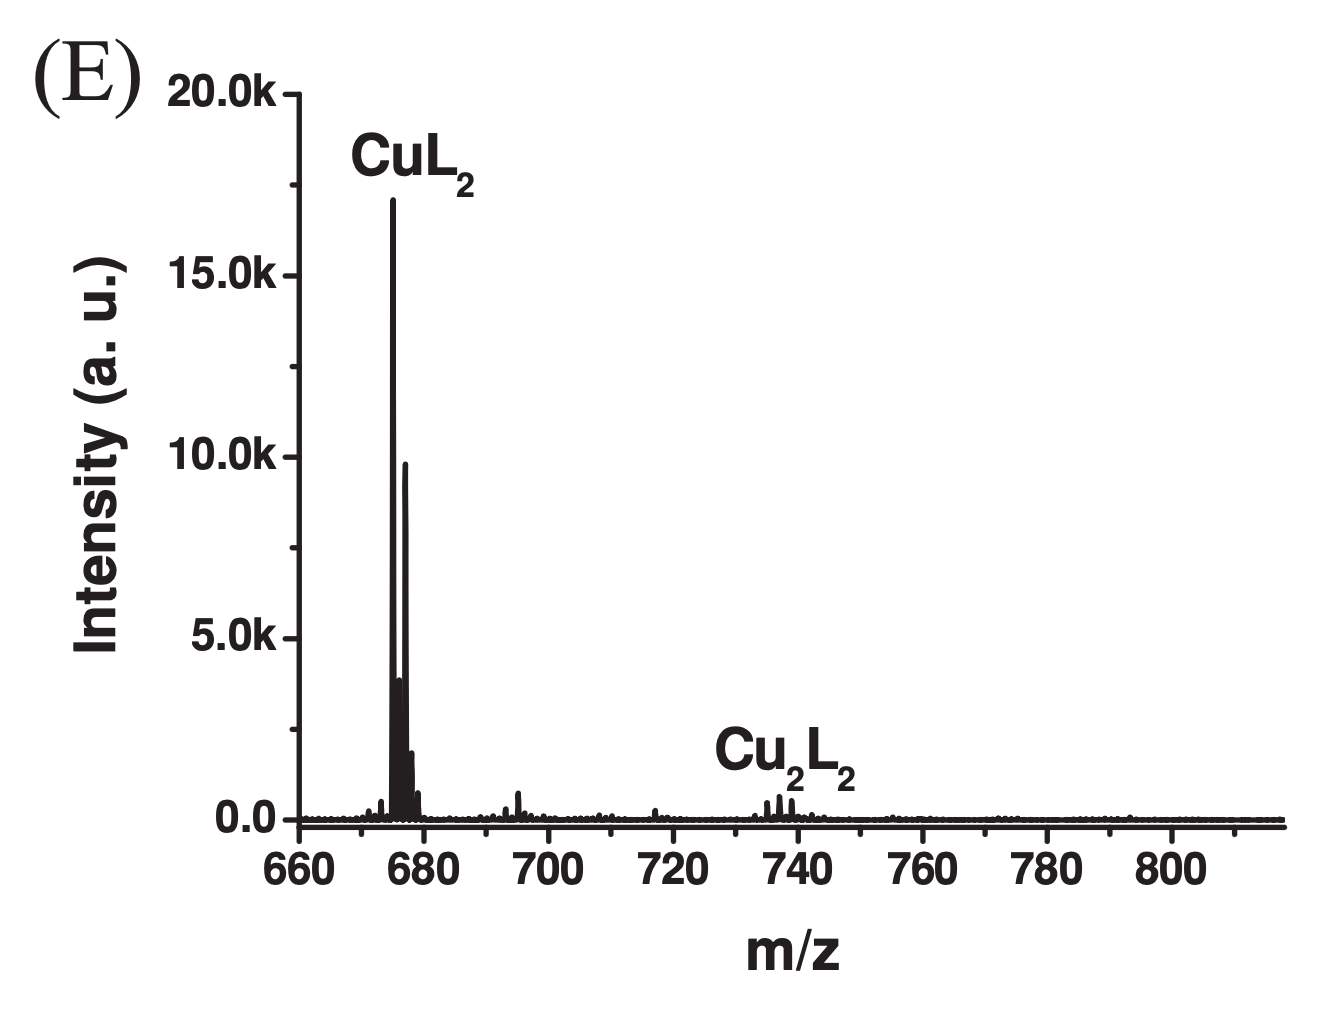
\includegraphics[width=0.7\linewidth]{pictures/cu_mass_spec.png}
	        \caption{\centering \scriptsize Масс-спектрометрия экспериментальных растворов Cys-CuNC. [1]}
	    \end{figure}
	    
	\column{0.5\textwidth}
	
		\begin{figure}
		    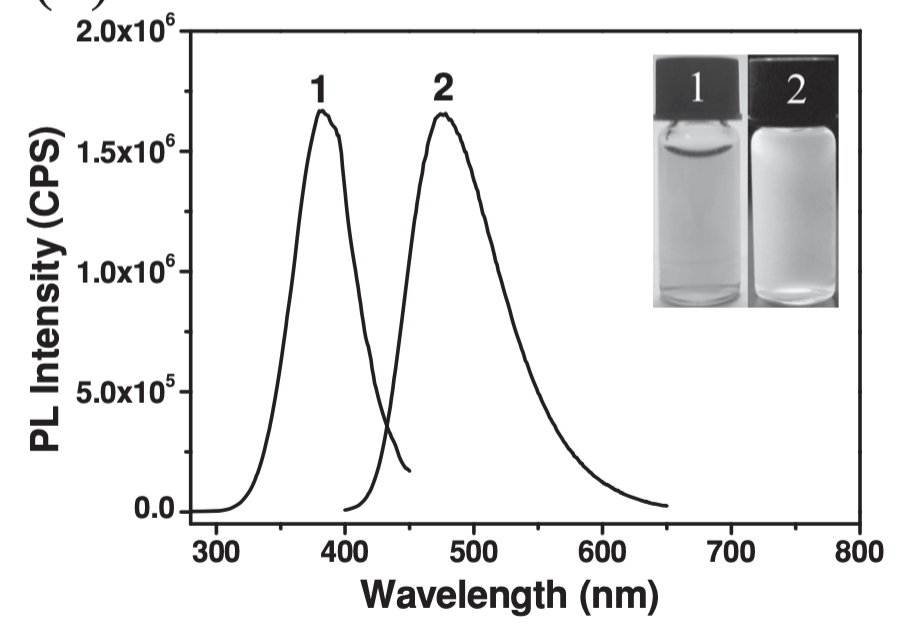
\includegraphics[width=0.9\linewidth]{pictures/abs_emm.png}
		    \caption{\centering \footnotesize Спектры возбуждения люминесценции (1) и испускания\ths (2) для Cys-CuNC. [1]}
		\end{figure}
		\vfill
		\tiny \textcolor{gray}{[1] Jia, X., Li, J., \& Wang, E. (2013). Cu nanoclusters with aggregation induced emission enhancement. Small, 9(22), 3873–3879. doi.org/10.1002/smll.201300896}
	\end{columns}
	
\end{frame}

\begin{frame}{Задачи работы}
	\justify
	Целью настоящей работы является определение структуры люминесцирующих кластеров. \\[0.5cm]
	
	% Целью настоящей работы является воспроизведение экспериментальных спектров поглощения и выявления оптимального метода расчёта. \\[0.5cm]
	
	Для достижения поставленной цели были сформулированы следующие задачи:
	\begin{enumerate}
		\item Построение геометрий комплексов \ce{[CuL2]^{-1}}, \ce{[Cu2L2]^{-2}}, \ce{[Cu3L2]^{-1}}, \ce{[Cu4L3]^{-1}} и \ce{[Cu5L4]^{-1}} (L — лиганд — \ce{SCH3} или Cys);
		\item Оптимизация геометрий комплексов;
		\item Расчёт референсных спектров поглощения и сравнительный анализ приближённых методов на основании комплексов с L — \ce{SCH3};
		\item Расчёт спектров поглощения для комплексов с цистеином. Сравнение с результатами для метилтиогруппы и экспериментальным спектром поглощения.
	\end{enumerate}
\end{frame}

\begin{frame}{Методы исследования}
	\justify
	Оптимизация структур проводилась при помощи метода теории возмущения MP2. Спектры поглощения расчитаны при помощи пяти гибридных DFT функционалов:
	\begin{enumerate}
		\item M06-2X;
		\item CAM-B3LYP;
		\item PBE0;
		\item $\omega$B97X;
		\item BHandHLYP.
	\end{enumerate}
	В качестве эталонного метода выбран метод связанных кластеров EOM-CCSD.
	\\
	На всех этапах использовался базис def2-TZVP.
	\\[0.5cm]
	Построение структур комплексов и визуализация результатов выполнены в программе \textbf{Chemcraft\ths1.8}. Оптимизация геометрии и моделирование спектров поглощения выполнены в программном пакете \textbf{ORCA 6.0}. Обработка спектров осуществлена в программе \textbf{OriginPro\ths2024}.
\end{frame}

\begin{frame}{Комплексы с метилтиогруппой. Оптимизация геометрии.}
	\begin{figure}[H]
		\centering
		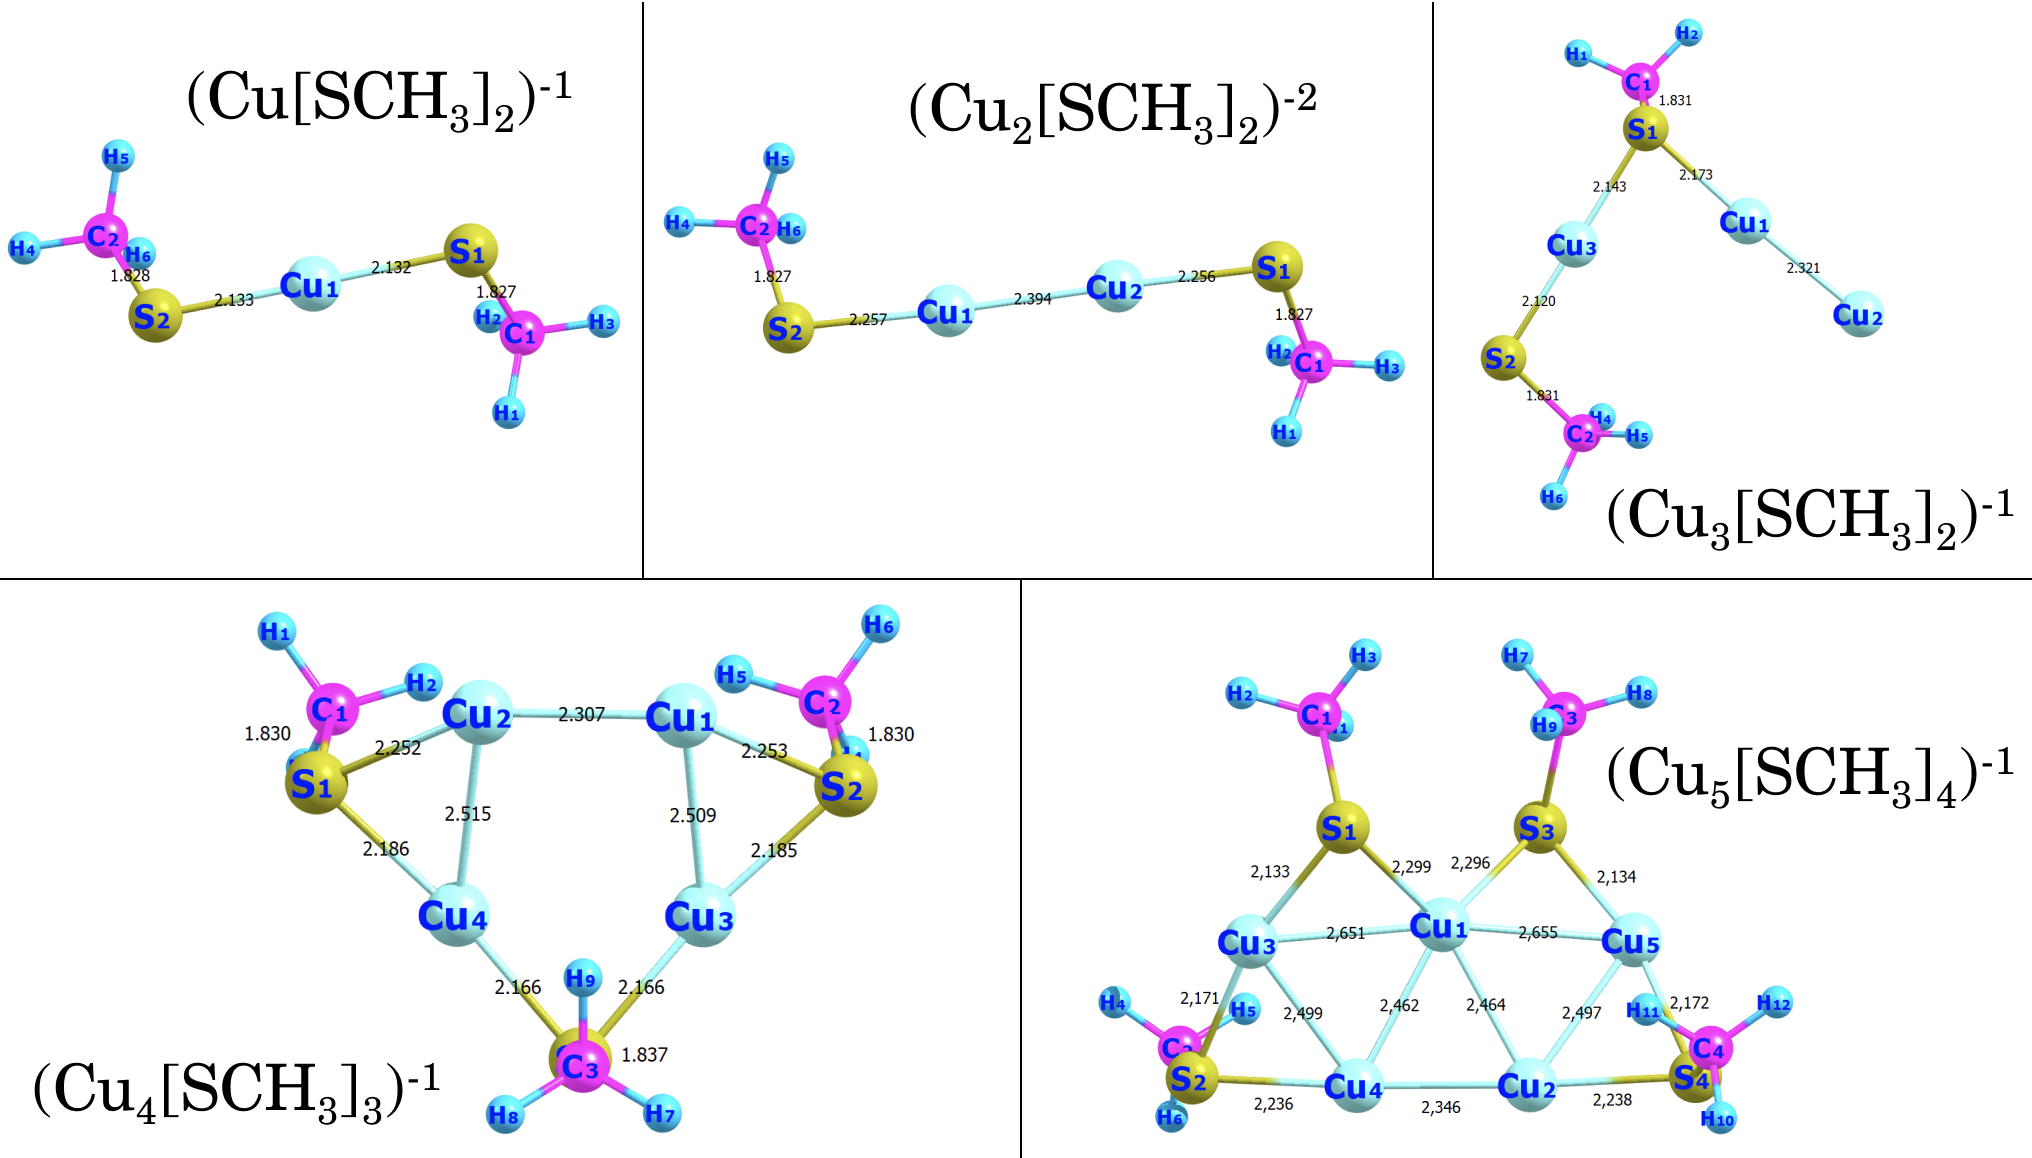
\includegraphics[width=0.75\textwidth, frame]{pictures/opt_SCH3_vac.jpg}
		\caption{\footnotesize Оптимизированные {в газовой фазе} геометрии комплексов, стабилизированных метилтиогруппой (метод: MP2/def2-TZVP).}
	\end{figure}
\end{frame}

\begin{frame}{Комплексы с метилтиогруппой. Сравнительный анализ спектров.}
	\begin{columns}
	
	\column{0.5\textwidth}
	
	\begin{figure}[H]
		\centering
		
\includegraphics[width=\textwidth]{pictures/spectra/Cu_vacuum.eps}
		\caption{\footnotesize Рассчитанные спектры поглощения для комплекса \ce{[Cu(SCH3)2]^{-1}} в газовой фазе.\\ Лоренцево уширение с полушириной 15\ths нм.}
	\end{figure}
	
	\column{0.5\textwidth}
	
	\begin{figure}[H]
		\centering
		
\includegraphics[width=\textwidth]{pictures/spectra/Cu2_vacuum.eps} 
		\caption{\footnotesize  Рассчитанные спектры поглощения для кластера \ce{[Cu2(SCH3)2]^{-2}} в газовой фазе.}
	\end{figure}
	
	\end{columns}
\end{frame}

\begin{frame}{Комплексы с метилтиогруппой. Сравнительный анализ спектров.}
	\begin{columns}
		
		\column{0.33\textwidth}
		
		\begin{figure}[H]
			\centering
			
\includegraphics[width=1.2\textwidth]{pictures/spectra/Cu3_vacuum.eps}
			\caption{\footnotesize Рассчитанные спектры поглощения для кластера \ce{[Cu3(SCH3)2]^{-1}} в газовой фазе.}
		\end{figure}
		
		\column{0.33\textwidth}
		
		\begin{figure}[H]
			\centering
			
\includegraphics[width=1.2\textwidth]{pictures/spectra/Cu4_vacuum.eps} 
			\caption{\footnotesize Рассчитанные спектры поглощения для кластера \ce{[Cu4(SCH3)3]^{-1}} в газовой фазе.}
		\end{figure}
		
		\column{0.33\textwidth}
		
		\begin{figure}[H]
			\centering
			
\includegraphics[width=1.2\textwidth]{pictures/spectra/Cu5_vacuum.eps}
			\caption{\footnotesize Рассчитанные спектры поглощения для кластера \ce{[Cu5(SCH3)4]^{-1}} в газовой фазе.}
		\end{figure}
		
	\end{columns}
\end{frame}

\begin{frame}{Комплексы с метилтиогруппой. Сравнительный анализ спектров.}
	\begin{columns}		
		\column{0.6\textwidth}
		
			\begin{table}[H]
				\caption{\scriptsize RMSE DFT-CCSD для всех переходов в эВ.}
				\label{tab_bench_1}
				\centering
				\footnotesize
				\begin{tabular}{|c|c|c|c|c|}
					\hline
					BHandH-LYP	&	CAM-B3LYP	& M06-2X	& PBE0	& wB97X	 	\\ \hline
					0,39		&   \textbf{0,25}		& 0,33		& 0,35	& 0,43	 	\\ \hline
				\end{tabular}
			\end{table}
			
			\begin{table}[H]
				\caption{\scriptsize RMSE DFT-CCSD для HOMO$\rarr$LUMO переходов в эВ.}
				\label{tab_bench_2}
				\centering
				\footnotesize
				\begin{tabular}{|c|c|c|c|c|}
					\hline
					BHandH-LYP	&	CAM-B3LYP	& M06-2X	& PBE0	& wB97X 	\\ \hline
					0,20		&   \textbf{0,17}		& 0,21		& 0,31	& 0,35 		\\ \hline
				\end{tabular}
			\end{table}	
		
		\column{0.4\textwidth}
		
			\begin{equation}
				\small
				RMSE = \sqrt{\frac{\sum\limits_{i=1}^N (E^{DFT}_i-E^{CCSD}_i)^2}{N}}
			\end{equation}
		
	\end{columns}
\end{frame}

\begin{frame}{Комплексы с метилтиогруппой. Сравнение с экспериментом.}
	\begin{columns}
		
		\column{0.5\textwidth}
		
		\begin{figure}[!h]
			\centering
			
\includegraphics[width=1\textwidth]{pictures/spectra/CAM-B3Lyp_vacuum.eps}
			\caption{\footnotesize Модельные спектры поглощения комплексов с метилтиогруппой, полученные при помощи метода \textbf{CAM-B3LYP}/def2-TZVP в газовой фазе.}
		\end{figure}
		
		\column{0.5\textwidth}
		
		\begin{figure}[H]
			\centering
			
\includegraphics[width=1\textwidth]{pictures/spectra/M06-2X_vacuum.eps} 
			\caption{\footnotesize Модельные спектры поглощения комплексов с метилтиогруппой, полученные при помощи метода \textbf{M06-2X}/def2-TZVP в газовой фазе.}
		\end{figure}
		
	\end{columns}
\end{frame}

\begin{frame}{\large Комплексы с метилтиогруппой. Спектр поглощения кластера \ce{[Cu2[SCH3]2]^{-2}}.}
	
	\begin{columns}
		
		\column{0.5\textwidth}
		
		\begin{figure}[!h]
			\centering
			\includegraphics[width=1\textwidth]{pictures/spectra/M06-2X_fix_vacuum.eps}
			\caption{\footnotesize Модельный спектр поглощения кластера \ce{[Cu2(SCH3)2]^{-2}}, полученные при помощи метода M06-2X/def2-TZVP в газовой фазе.\\ Гауссово уширение с полушириной 50\ths нм.}
		\end{figure}
		
		\column{0.5\textwidth}
		
		\begin{figure}[!htb]
			\centering
			
			\subfloat[Переход 2px$\rarr$2py (396,1\ths нм)]{ 
\includegraphics[clip,width=0.5\columnwidth]{pictures/orbitals/Cu2L2_1.jpg} }
			\subfloat[Переход 2px$\rarr$3pz (373,4\ths нм)]{ 
\includegraphics[clip,width=0.5\columnwidth]{pictures/orbitals/Cu2L2_2.jpg} }
			
			\subfloat[Переход 2px$\rarr$3px (365,3\ths нм)]{ 
\includegraphics[clip,width=0.5\columnwidth]{pictures/orbitals/Cu2L2_3.jpg} }
			
			\caption{\footnotesize Основные вклады в спектр поглощения кластера \ce{[Cu2(SCH3)2]^{-2}} в газовой фазе.\\ Проекция изоповерхностей электронной плотности. Метод M06-2X/def2-TZVP.}
		\end{figure}
		
	\end{columns}
	
	
\end{frame}

\begin{frame}{Комплексы с цистеином. Оптимизация геометрии.}
	\begin{figure}[H]
		\centering
		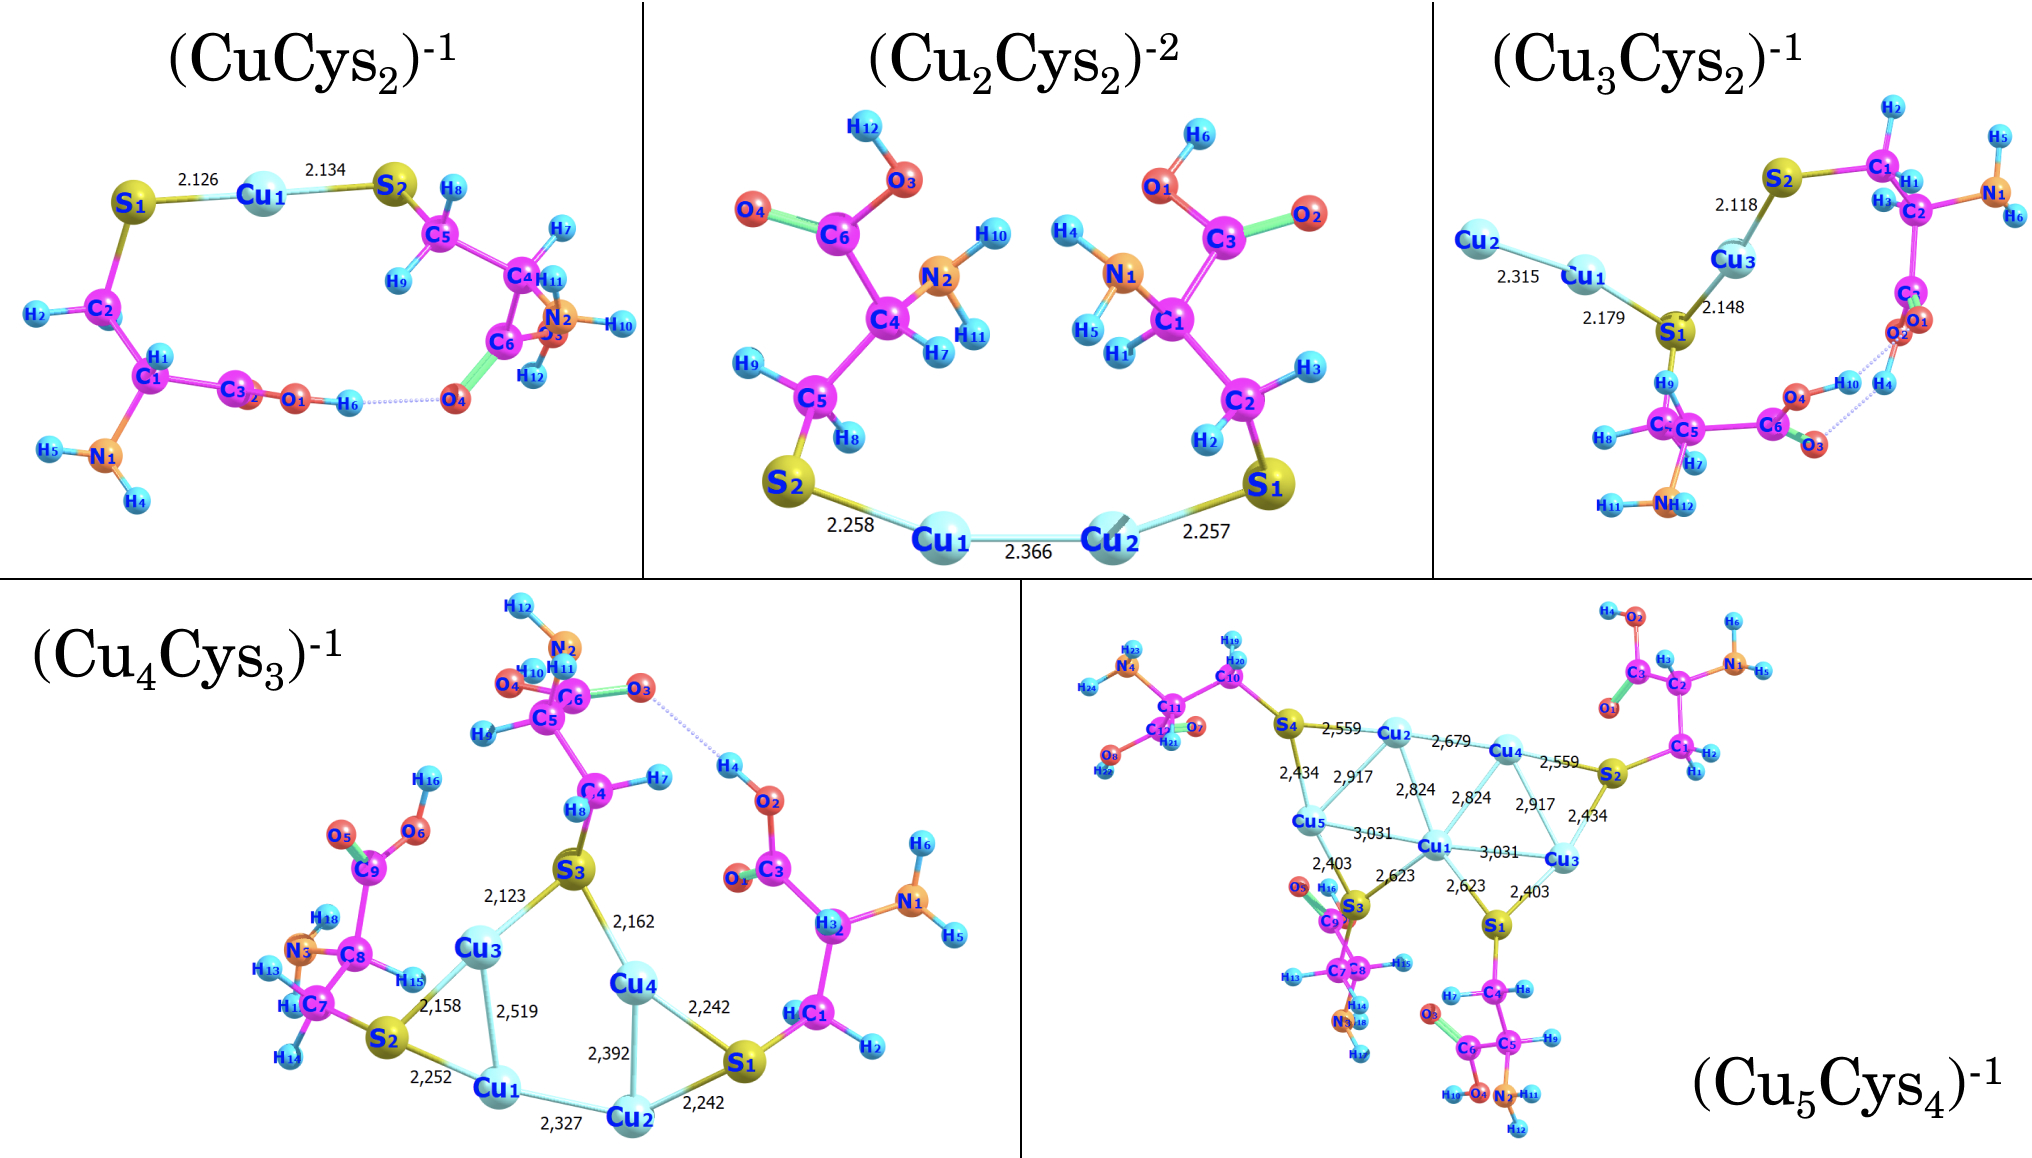
\includegraphics[width=0.75\textwidth, frame]{pictures/opt_Cys_vac.jpg}
		\caption{\footnotesize Оптимизированные {в газовой фазе} геометрии комплексов, стабилизированных цистеином (метод: MP2/def2-TZVP).}
	\end{figure}
	
%	Замена метилтиогруппы на цистеиновый фрагмент действительно приводит к изменениям геометрии комплексов. Однако степень этих изменений существенно зависит от конкретной структуры: в одних случаях они оказываются минимальными, тогда как в других становятся более выраженными и заметными.

%	Следует подчеркнуть, что даже в худших случаях изменение геометрических параметров остается ограниченным: длины валентных связей отличаются не более чем на 0,4Å, а валентные углы — не более чем на 20º. При этом подобные значения можно рассматривать скорее как исключения из общей тенденции. В среднем же замена лиганда на цистеин приводит к значительно меньшим изменениям: длины связей варьируются не более чем на 0,1Å, а изменения валентных углов, как правило, не превышают 10º.
\end{frame}

\begin{frame}{Комплексы с цистеином. Сравнение с экспериментом.}
	\begin{columns}
		
		\column{0.5\textwidth}
		
		\begin{figure}[!h]
			\centering
			
\includegraphics[width=1\textwidth]{pictures/spectra/Cys_CAM-B3Lyp_vacuum.eps}
			\caption{\footnotesize Модельные спектры поглощения комплексов с цистеином, полученные при помощи метода \textbf{CAM-B3LYP}/def2-TZVP в газовой фазе.}
		\end{figure}
		
		\column{0.5\textwidth}
		
		\begin{figure}[H]
			\centering
			
\includegraphics[width=1\textwidth]{pictures/spectra/Cys_M06-2X_vacuum.eps} 
			\caption{\footnotesize Модельные спектры поглощения комплексов с цистеином, полученные при помощи метода \textbf{M06-2X}/def2-TZVP в газовой фазе.}
		\end{figure}
		
	\end{columns}
\end{frame}

\begin{frame}{Выводы}
	\begin{enumerate}
		\item По результатам сравнительного анализа предпочтительным методом для расчёта спектров поглощения (электронных переходов) является метод M06-2X. Хотя CAM-B3LYP дал лучшую сходимость с EOM-CCSD, он не показал такого же хорошего согласования с экспериментальным спектром поглощения.
		\item Замена метилтиогруппы на цистеин приводит к изменениям геометрии комплексов. Однако степень этих изменений существенно зависит от конкретной структуры: в одних случаях они оказываются минимальными, тогда как в других становятся более выраженными и заметными.
		\item Спектры поглощения, полученные методом M06-2X/def2-TZVP, подтверждают данные масс-спектрометрии раствора медных НК с цистеином. Наибольший вклад в спектры возбуждения люминесценции вносит кластер \ce{[Cu2L_2]^{-2}}. Комплекс \ce{[CuL_2]^{-1}} также может присутствовать в растворе в большом количестве, так как его спектр лежит в более коротковолновой области.
	\end{enumerate}
\end{frame}

\begin{frame}{Практическая значимость работы}
	\begin{itemize}
		\item Результаты работы могут быть использованы для создания новых диагностических инструментов, нацеленных на обнаружение тиолятов, например в сыворотке крови человека \textit{in vitro}. 
		\item Предсказуемые спектры поглощения систем позволят в будущем оценить взаимодействие таких биосенсоров с органическими молекулами, что обеспечит мишенепривязанность.
		\item Результаты сравнительного анализа позволят ускорить расчёт аналогичных серосодержащих систем.
	\end{itemize}
	
	\vfill
	Дальнейшее продолжение работы может включать: 
	\begin{enumerate}
		\item Рассмотрение кластеров меди с другими тиолами (глутатион, кофермент А и\ths пр.);
		\item Анализ стабильности систем (энергии комплексообразования). 
		%Хотя известно, что комплексы можно экспериментально синтезировать, расчёт энергии комплексообразования может дать дополнительную информацию о стабильности таких структур;
		\item Расчёт спектров поглощения с явным учётом растворителя. %Континуальная модель CPCM не обеспечила хороших результатов. Учёт растворителя в явном виде (например при помощи ONIOM) может исправить ситуацию
	\end{enumerate}	
	
\end{frame}

\begin{frame}{Благодарности}
	\small 
	\begin{itemize}
		\item Выражаю особую благодарность моему научному руководителю, кандидату химических наук, старшему научному сотруднику кафедры Молекулярной биофизики и физики полимеров Физического факультета СПбГУ, Буглаку Андрею Андреевичу, за всеобъемлющую помощь в ходе проведения данного исследования.
		\item Выражаю благодарность кандидату физико-математических наук, старшему научному сотруднику кафедры Молекулярной биофизики и физики полимеров Физического факультета СПбГУ, Сычу Томашу Сергеевичу за помощь в подготовке оборудования для проведения квантово-химических расчетов исследуемых структур.
		\item Выражаю благодарность кандидату физико-математических наук Помогаеву Владимиру Анатольевичу за консультации по работе с программными пакетами для квантово-химических вычислений.
		\item Выражаю благодарность Кононову Алексею Игоревичу, доктору физико-математических наук, руководителю научной группы Биофотоники (\href{https://biophotonics.spbu.ru}{https://biophotonics.spbu.ru}).
		\item Выражаю отдельную благодарность своим родителям за вклад в моё образование и воспитание. Без них я бы не смог преодолеть все трудности обучения на Физфаке.
	\end{itemize}
	\vfill
	\footnotesize{Работа выполнена с использованием оборудования Ресурсного Центра СПбГУ «Вычислительный Центр».}
\end{frame}

\begin{frame}[plain]
	\centering
	\huge{\textbf{Спасибо за внимание!}} 
\end{frame}

\begin{frame}{К ответу на вопрос рецензента}
	\begin{columns}
		\column{0.5\textwidth}
		\begin{figure}
			\centering
			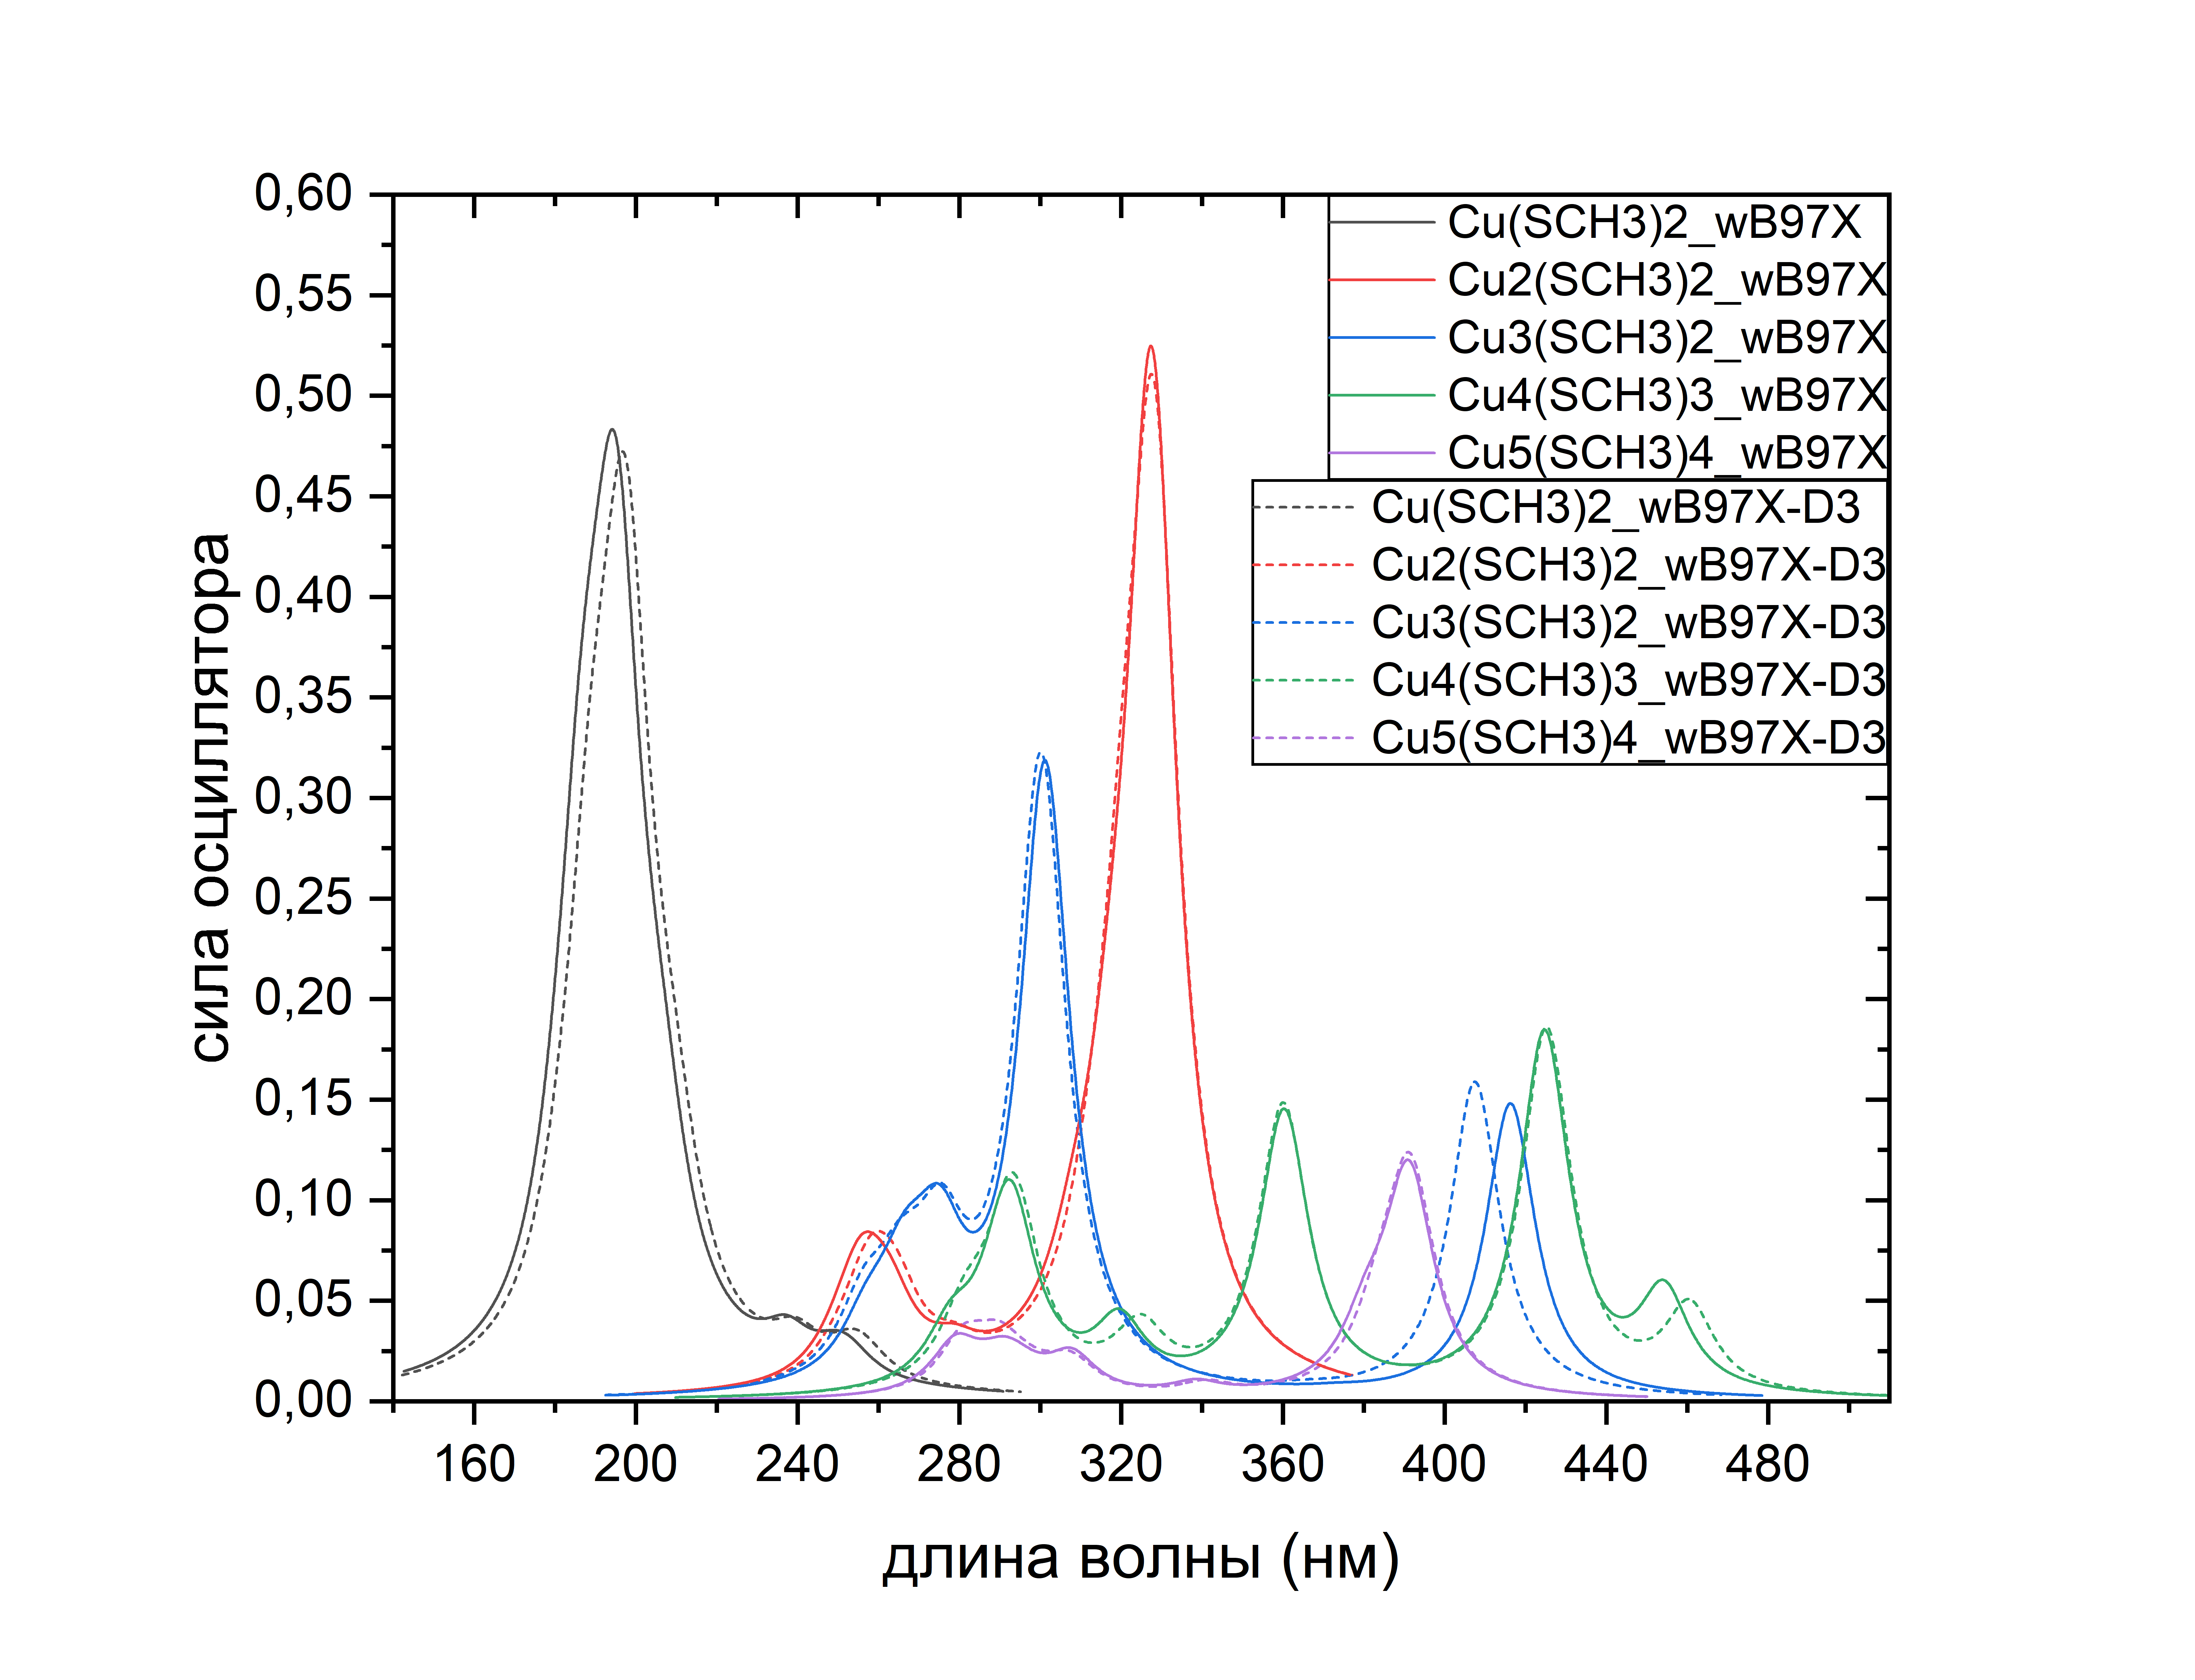
\includegraphics[width=1\textwidth]{pictures/spectra/exci_wB97X-D3_vacuum.eps} 
			\caption{\footnotesize Модельные спектры поглощения комплексов с метилтиогруппой, полученные при помощи методов wB97X и wB97X-D3 в газовой фазе. Лоренцево уширение с полушириной 15\ths нм.}
		\end{figure}
		
		\column{0.5\textwidth}
		
		\begin{table}[H]
			\caption{\scriptsize RMSE DFT-CCSD для всех переходов в эВ.}
			\label{tab_bench_3}
			\centering
			\footnotesize
			\begin{tabular}{|c|c|}
				\hline
				wB97X	& wB97X-D3	\\ \hline
				0,43	& 0,42		\\ \hline
			\end{tabular}
		\end{table}
		
		\begin{table}[H]
			\caption{\scriptsize RMSE DFT-CCSD для HOMO$\rarr$LUMO переходов в эВ.}
			\label{tab_bench_4}
			\centering
			\footnotesize
			\begin{tabular}{|c|c|}
				\hline
				wB97X	& wB97X-D3	\\ \hline
				0,35	& 0,32		\\ \hline
			\end{tabular}
		\end{table}	
		
	\end{columns}
	
\end{frame}

\end{document}



